\documentclass[11pt]{article}

\usepackage{amsmath,amssymb}
\usepackage{graphicx}
\usepackage{hyperref}
\usepackage{tikz}
\usetikzlibrary{arrows.meta,positioning}

\title{PLN as a Common Substrate for Naive Bayes and k-NN Premise Selection}
\author{Mettapedia Working Notes}
\date{\today}

\begin{document}
\maketitle

\begin{abstract}
We treat evidence as a first-class object and show how the core PLN operations
(tensor and revision) subsume two classical premise selectors: Naive Bayes (NB)
and k-nearest neighbors (k-NN), and compose them into novel architectures.
The NB bridge is formalized in Lean; the
k-NN bridge is added as a direct evidence aggregation that matches the MaSh
relevance formula. We isolate the MaSh instance (IDF weights, nearness, and
relevance) as a specialization of the general k-NN scheme, and we record clean
optimality-transfer lemmas that let PLN inherit NB/k-NN guarantees under explicit
assumptions. We prove that PLN revision (hplus) is the \emph{unique}
evidence-level pooling operator satisfying external Bayesianity and total
additivity, correcting a gap in the classical axiomatization via an explicit
counterexample. Experimentally, on round-2 pooled-data validation runs
(E prover, 5s, no \texttt{-p}), the best top-256 result is 290/800 (MaSh NB)
and the best PLN result is 288/800 (mixture-local Prior$\otimes$NB); at top-512,
MaSh k-NN and PLN mixture-local Prior$\otimes$NB tie at 286/800.
\end{abstract}

\section{High-level picture}
PLN treats truth values as evidence pairs $(n^+,n^-)$ and composes them in two
ways:

\begin{itemize}
\item \textbf{Tensor} (sequential composition) multiplies evidence.
\item \textbf{Revision} (``hplus'') adds evidence from independent sources.
\end{itemize}

NB and k-NN both arise as instances of these primitives:

\begin{itemize}
\item NB: tensor-multiply feature evidence, then read off a posterior via
      the strength map.
\item k-NN: revise (hplus) per-neighbor relevance evidence; the total positive
      evidence is exactly the k-NN relevance score.
\end{itemize}

\begin{figure}[h]
\centering
\resizebox{\linewidth}{!}{
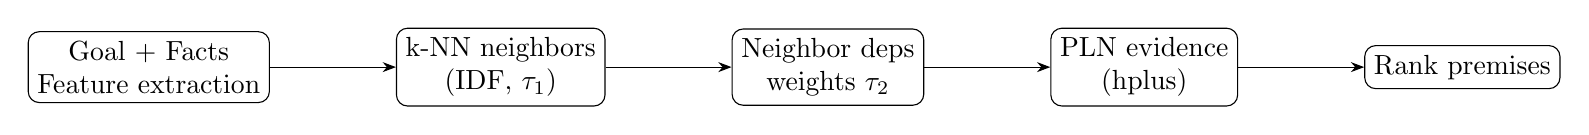
\begin{tikzpicture}[node distance=16mm,>=Stealth]
  \node (feat) [draw,rounded corners,align=center] {Goal + Facts\\Feature extraction};
  \node (knn) [draw,rounded corners,align=center,right=of feat] {k-NN neighbors\\(IDF, $\tau_1$)};
  \node (deps) [draw,rounded corners,align=center,right=of knn] {Neighbor deps\\weights $\tau_2$};
  \node (pln) [draw,rounded corners,align=center,right=of deps] {PLN evidence\\(hplus)};
  \node (rank) [draw,rounded corners,align=center,right=of pln] {Rank premises};
  \draw[->] (feat) -- (knn);
  \draw[->] (knn) -- (deps);
  \draw[->] (deps) -- (pln);
  \draw[->] (pln) -- (rank);
\end{tikzpicture}
}
\caption{k-NN scoring as PLN evidence aggregation.}
\end{figure}

\section{Feature sets and IDF}
Given a finite set of facts $\Phi$, a feature extractor $F : \Phi \to \mathcal{P}(\mathcal{F})$,
we define the IDF weight
\[
  w(f,\Phi) = \log\left(\frac{|\Phi|}{|\{\varphi\in\Phi : f\in F(\varphi)\}|}\right).
\]

In Lean, the general definitions are in
\texttt{Mettapedia/Logic/PremiseSelectionKNN.lean}.

\section{k-NN relevance and the MaSh instance}
Define nearness
\[
  n(\varphi,\chi) = \sum_{f \in F(\varphi) \cap F(\chi)} w(f)^{\tau_1}.
\]
The MaSh k-NN relevance for a goal $\gamma$ is
\[
  R(\varphi,\gamma) = \begin{cases}
    \tau_2\sum_{\chi\in N} \mathbf{1}[\varphi\in \mathrm{deps}(\chi)]\,\frac{n(\chi,\gamma)}{|\mathrm{deps}(\chi)|}
      + n(\varphi,\gamma), & \varphi\in N \\
    0, & \text{otherwise.}
  \end{cases}
\]

This is formalized in Lean as:
\begin{itemize}
\item \texttt{knnNear}, \texttt{knnScoreTopK} (general k-NN)
\item \texttt{mashNear}, \texttt{mashScoreTopK} (MaSh instance)
\item \texttt{knnRelevanceENN\_paper} (ENNReal paper-style form)
\item \texttt{knnRelevanceENN\_eq\_paper} (proof of equivalence)
\end{itemize}

\section{PLN bridge for k-NN}
Let $\mathrm{posEvidence}(x) = (x,0)$ and combine independent evidence via
$\oplus$ (hplus). For each neighbor $\chi$ we create a positive evidence
contribution for each dependent $\varphi$ proportional to
$\tau_2\,n(\chi,\gamma)/|\mathrm{deps}(\chi)|$. We then hplus all contributions
and (optionally) add the self-neighbor term.

In Lean, we define
\texttt{plnKnnEvidence} and prove:
\[
  (\text{plnKnnEvidence}\;\gamma\;N\;\dots\;\varphi).pos
  = \text{knnRelevanceENN}(\gamma,N,\dots,\varphi).
\]
This is the formal PLN--kNN bridge.

\section{PLN bridge for Naive Bayes}
The PLN NB bridge is already formalized in
\texttt{Mettapedia/Logic/PLNBayesNetInference.lean}:

\begin{itemize}
\item \texttt{nbEvidence} multiplies feature evidence via tensor.
\item \texttt{toStrength\_nbEvidence\_eq\_nbPosterior} shows the PLN evidence view
      equals textbook NB posterior.
\end{itemize}

This links the PLN evidence calculus directly to a standard NB classifier.

\section{Optimality transfer (NB, k-NN, and PLN)}
We record minimal, assumption-explicit transfer lemmas in
\texttt{Mettapedia/Logic/PremiseSelectionOptimality.lean}:

\begin{itemize}
\item \texttt{nb\_optimal\_of\_zhang}: if the NB score equals the Bayes posterior,
      then the NB classifier is Bayes-optimal.
\item \texttt{nb\_ranking\_of\_zhang\_su}: if the NB score is a strict monotone
      transform of the posterior, then its ranking is Bayes-optimal.
\item \texttt{knn\_ranking\_of\_consistency}: if k-NN converges to the posterior,
      its ranking is Bayes-optimal.
\item \texttt{pln\_inherits\_nb\_optimal}, \texttt{pln\_inherits\_nb\_ranking},
      \texttt{pln\_inherits\_knn\_ranking}: PLN emulation inherits optimality when
      its score matches the base method.
\item \texttt{ranking\_optimal\_of\_linear\_combo}: positive linear combinations of
      strict monotone transforms of the posterior preserve optimal ranking.
\item \texttt{fusion\_ranking\_of\_linear\_combo}: if fusion reduces to a positive
      linear combination of two monotone scores, the fused ranking is optimal.
\item \texttt{fusion\_ranking\_after\_normalization}: same statement, but named to
      emphasize the normalization pathway used to fix evidence totals.
\item \texttt{fusion\_ranking\_after\_normalization\_toReal} and
      \texttt{fusion\_ranking\_after\_normalization\_toReal\_one} provide the
      real-valued ranking corollary, with a no-hassle $t=1$ specialization.
\item \texttt{rankingENN\_toReal}: drop ENNReal coercion gaps by transferring ranking
      optimality to real-valued scores under finiteness assumptions.
\end{itemize}

\section{Fusion (NB + k-NN) via PLN revision}
To leverage both methods, we fuse their Evidence-valued scores by PLN revision
($\oplus$ / hplus). The key theorem in
\texttt{Mettapedia/Logic/PremiseSelectionFusion.lean} states that the strength
of the fused score is a \emph{weighted average} of the component strengths:
\[
  s(E_1 \oplus E_2) =
  \frac{w_1}{w_1+w_2} s(E_1) + \frac{w_2}{w_1+w_2} s(E_2),
\]
where $w_i$ is the total evidence of $E_i$ and $s$ is the PLN strength view.
This is exactly the revision rule from the PLN book, now used as a clean
mathematical unifier for premise-selection ensembles.

We also record a constant-weight specialization:
\texttt{fuse\_toStrength\_const\_weights} shows that if evidence totals are fixed
across candidates, the fused score is a fixed convex combination of the base
scores, enabling direct ranking-transfer lemmas.
More generally, \texttt{fuse\_toStrength\_proportional\_weights} shows that if
both evidence totals share a common per-candidate factor, the factor cancels and
the fusion still reduces to a constant convex combination.
We additionally normalize evidence totals when needed:
\texttt{normalizeEvidence} / \texttt{normalizeScorer} fix the total to a chosen
$t$ while preserving strength, and
\texttt{fuse\_toStrength\_normalized\_const\_toReal} yields the real-valued
convex combination used in
\texttt{fusion\_ranking\_after\_normalization\_toReal}.

\section{External-Bayesianity: Counterexample and Corrected Uniqueness}
The external-Bayesian commutation law
\[
  \mathrm{update}(\mathrm{fuse}(s_1,s_2),\ell)
  =
  \mathrm{fuse}(\mathrm{update}(s_1,\ell),\mathrm{update}(s_2,\ell))
\]
is algebraically exact in our evidence semiring (distributivity of tensor over hplus).
However, this law alone does \emph{not} characterize additive pooling.

\subsection{Counterexample under the original pooling axioms}
In \texttt{Mettapedia/Logic/PremiseSelectionExternalBayesianity.lean}, we define
\texttt{maxPoolingOperator} (coordinatewise max on evidence pairs) and prove
\texttt{maxPoolingOperator\_ne\_fuse}.  Thus, commutativity, associativity, neutrality,
and external-Bayesianity do not force \texttt{pool = fuse}.

\subsection{Corrected uniqueness theorem}
We then add the missing PLN-semantic axiom: \emph{total additivity}
(\texttt{total(pool(x,y)) = total(x)+total(y)}).  Using tensor masks
\(\langle 1,0\rangle\) and \(\langle 0,1\rangle\), we prove:
\begin{itemize}
\item \texttt{poolE\_eq\_hplus\_of\_externalBayes\_totalAdd}:
      external-Bayesianity + total-additivity force coordinatewise addition at
      the evidence level.
\item \texttt{poolingOperator\_pointwise\_unique\_of\_externalBayes\_totalAdd}:
      scorer-level uniqueness to \texttt{fuse}, given a pointwise lift
      \((P.pool\,s_1\,s_2)(g,f)=\mathrm{poolE}(s_1(g,f),s_2(g,f))\).
\item \texttt{not\_fuse\_of\_no\_pointwise\_lift}:
      if a scorer-level pooling operator admits no pointwise evidence kernel,
      it cannot be equal to \texttt{fuse}.
\end{itemize}

\section{Quantitative finite-mixture TV bounds}
The finite local-mixture bridge in
\texttt{Mettapedia/Logic/PremiseSelectionLocalMixtureBridge.lean}
now includes:
\begin{itemize}
\item \texttt{finite\_statistic\_tv\_mixture\_bound}: unconditional TV-style bound
      from the existing finite iid-vs-injective L1 estimate.
\item \texttt{finite\_binary\_statistic\_tv\_mixture\_bound}: binary
      (\texttt{used}/\texttt{not-used}) specialization.
\item \texttt{finite\_statistic\_tv\_mixture\_bound\_choose2\_of\_l1}:
      tight-constant transfer form: if
      \(L_1 \le m(m-1)/R\), then
      \(\mathrm{TV} \le m(m-1)/(2R)\).
\item \texttt{l1\_iid\_inj\_le\_choose2} (in
      \texttt{Mettapedia/Logic/DiaconisFreedmanFinite.lean}):
      unconditional base collision bound
      \(L_1 \le m(m-1)/R\).
\item \texttt{finite\_statistic\_tv\_mixture\_bound\_choose2}:
      unconditional tight TV theorem obtained by composing the transfer form
      with \texttt{l1\_iid\_inj\_le\_choose2}.
\item \texttt{finite\_statistic\_tv\_mixture\_bound\_m16\_R4551} and
      \texttt{finite\_binary\_statistic\_tv\_mixture\_bound\_m16\_R4551}:
      concrete premise-selection instantiation for neighborhood size \(m=16\)
      and axiom pool size \(R=4551\), yielding
      \(\mathrm{TV} \le 120/4551 \approx 0.0264\).
\end{itemize}
This separates (i) the transport theorem to pushed-forward statistics from
(ii) the combinatorial collision estimate used to supply the base L1 constant,
now in a fully unconditional tight-constant form.

\subsection{Three-Pillar Theorem Summary}
For the Prior-NB selector family, the formal story is now organized into three
pillars that match implementation semantics:
\begin{itemize}
\item \textbf{Role discipline (prior vs likelihood):}
      \texttt{OperatorRoleTheory}, \texttt{posterior\_eq\_twoStage}, and
      \texttt{priorNBPosterior\_eq\_twoStage} enforce that prior sources are
      pooled via revision (\texttt{fuse}/hplus) and feature evidence is composed
      via tensor (\texttt{update}). For traceability aliases, see
      \texttt{PLN\_LocalEvidenceRevision},
      \texttt{PLN\_NormalizedSequentialComposition}, and
      \texttt{PLN\_StrengthRankingPreservation} in
      \texttt{PremiseSelectionPriorNB.lean}.
\item \textbf{Corrected pooling uniqueness:}
      \texttt{maxPoolingOperator\_ne\_fuse} gives a concrete counterexample under
      the old axioms, while
      \texttt{poolE\_eq\_hplus\_of\_externalBayes\_totalAdd} proves uniqueness
      once total-additivity is added.
\item \textbf{Finite local-mixture approximation:}
      \texttt{finite\_statistic\_tv\_mixture\_bound\_choose2} and
      \texttt{finite\_statistic\_tv\_mixture\_bound\_m16\_R4551} provide explicit
      finite-sample control for the neighborhood regime used in our selectors.
\end{itemize}
These theorems target \emph{surrogate ranking quality} (coverage / Bayes-optimal
ranking transfer), which is the right formal objective for premise selection.
They do not claim direct guarantees on ATP wall-clock solve rates, which remain
an empirical systems-level outcome.

\section{Round-2 experimental validation on extended MPTP 5k}
\subsection{Protocol and data integrity}
We evaluate seven selectors under one canonical protocol:
\begin{itemize}
\item Dataset: 4200 train problems, 800 validation problems.
\item Model-generation data source: pooled dependency events
      (\texttt{pooled\_train\_deps\_allruns.jsonl}), built from base train deps
      plus prior train proof runs; final pool size is 9045 events over 1649 unique
      training problems.
\item Selection budgets: top-256 and top-512.
\item Prover route: E 3.0.1-ho, timeout 5s, jobs=4, \emph{without} E's \texttt{-p}.
\item Integrity policy: generate top-512 selections first, derive top-256 by prefix
      truncation, then run E on both budgets.
\end{itemize}

\subsection{Methods in PLN rule style}
In the PLN book spirit, we keep evidence as the primary object and use only:
revision (\(\oplus\), evidence accumulation), tensor (\(\otimes\), sequential
composition), and normalization (fix evidence mass while preserving strength).

For the new mixture-local selector (\texttt{select\_pln\_mixture\_local\_nb.py}),
the staged construction is:
\[
  E_{\text{post}}(g,a) =
  \Big(
    \bigoplus_i \mathrm{Normalize}_{t_i(g)}(E_i^{\text{local}}(g,a))
    \oplus \mathrm{Normalize}_{t_G}(E^{\text{global}}(a))
  \Big)\otimes
  \mathrm{Normalize}_{t_L}(E^{\text{NB-like}}(g,a)).
\]
Here each local expert \(i\) is built from a k-NN bin:
\[
  n_i^+(g,a)=\sum_{\chi\in B_i(g)} \mathrm{sim}(g,\chi)\,\mathbf{1}[a\in deps(\chi)],
\]
\[
  n_i^-(g,a)=\eta\sum_{\chi\in B_i(g)} \mathrm{sim}(g,\chi)\,\mathbf{1}[a\notin deps(\chi)].
\]
We use \(E_i^{\text{local}}=(n_i^++\alpha,\;n_i^-+\beta)\), with weak-negative
factor \(\eta=0.08\), bins \([4,16,64,256]\), and similarity
\(\mathrm{sim}=\mathrm{overlap}/(\mathrm{overlap}+\kappa)\).
Likelihood evidence is \emph{NB-likelihood only} (prior removed by setting
\(\sigma_1=0\)), then robustly scaled per problem (IQR target) before conversion
to odds evidence and normalization.

This gives a non-alias architecture:
\begin{itemize}
\item Stage A: multiple local priors from neighbor bins.
\item Stage B: normalized pooling via revision (\(\oplus\)).
\item Stage C: normalized tensor with likelihood-only NB evidence.
\end{itemize}

\subsection{Round-1 reference results}
To keep the chronology explicit, Table~\ref{tab:r1val} lists the pre-pooled
round-1 validation runs used before the round-2 pooled-data refresh.

\begin{table}[h]
\centering
\begin{tabular}{lrr}
\hline
Model (round1 reference) & Top-256 & Top-512 \\
\hline
MaSh NB & 283/800 (35.38\%) & 291/800 (36.38\%) \\
PLN kNN-prior-NB (opt, merge-NB) & 282/800 (35.25\%) & 291/800 (36.38\%) \\
PLN NB & 281/800 (35.12\%) & n/a \\
PLN Normal-NB & 279/800 (34.88\%) & n/a \\
PLN Enhanced & 276/800 (34.50\%) & n/a \\
MaSh k-NN & 272/800 (34.00\%) & 291/800 (36.38\%) \\
\hline
\end{tabular}
\caption{Round-1 validation reference results (legacy pre-pooled run set).}
\label{tab:r1val}
\end{table}

\subsection{Validation results (canonical 14 runs)}
Table~\ref{tab:r2val} reports all seven models at top-256 and top-512.

\begin{table}[h]
\centering
\begin{tabular}{lrr}
\hline
Model (round2\_pooled) & Top-256 & Top-512 \\
\hline
MaSh NB & 290/800 (36.25\%) & 285/800 (35.63\%) \\
PLN mixture-local Prior$\otimes$NB & 288/800 (36.00\%) & 286/800 (35.75\%) \\
PLN kNN-prior-NB (opt, merge-NB) & 281/800 (35.12\%) & 285/800 (35.63\%) \\
MaSh k-NN & 280/800 (35.00\%) & 286/800 (35.75\%) \\
PLN Normal-NB & 280/800 (35.00\%) & 282/800 (35.25\%) \\
PLN NB & 276/800 (34.50\%) & 285/800 (35.63\%) \\
PLN Enhanced & 272/800 (34.00\%) & 283/800 (35.38\%) \\
\hline
\end{tabular}
\caption{Round-2 validation results (E5s, no-\texttt{-p}, jobs=4).}
\label{tab:r2val}
\end{table}

\subsection{Discussion}
\begin{itemize}
\item \textbf{Top-256 precision regime}: MaSh NB is best (290), but the new
      PLN mixture-local model is very close (288). The margin is 2/800.

\item \textbf{Top-512 recall regime}: MaSh k-NN and PLN mixture-local tie for best
      (286), with MaSh NB and two PLN variants at 285. At this budget, differences
      are effectively tie-level.

\item \textbf{Overlap is high}: at top-256, MaSh NB and PLN mixture-local share
      287 solved problems, with only 3 NB-unique and 1 mixture-unique. At top-512,
      MaSh NB vs MaSh k-NN differs on just 5 problems total.

\item \textbf{Greedy-cover complementarity remains small but real}: top-5 greedy
      union is 297 solved with all runs, and 296 without MaSh runs. So MaSh adds
      one extra unique solve in this top-5 cover view.

\item \textbf{PLN interpretation}: these results match the formal story. Revision
      and tensor composition are structurally correct, but empirical gains depend on
      calibration quality of local priors and gating, not on operator choice.
\end{itemize}

\subsection{Implementation notes}
\begin{itemize}
\item PeTTa-backed selectors:
      \texttt{select\_pln\_nb.py},
      \texttt{select\_pln\_normal\_nb.py},
      \texttt{select\_pln\_enhanced.py},
      \texttt{select\_pln\_knn\_prior\_nb\_opt.py}
      (using \texttt{hyperon/PeTTa/demos/pln\_*\_selector*.metta} and
      \texttt{hyperon/PeTTa/lib/lib\_pln\_xi.metta}).
\item Pure-Python selector:
      \texttt{select\_pln\_mixture\_local\_nb.py}
      (same evidence algebra, staged explicitly for auditability/performance).
\item Round-2 queue/orchestration:
      \texttt{atps/scripts/queue\_round2\_val\_e5\_nop.sh}.
\item Compact scoreboard and greedy cover artifacts:
      \texttt{results\_round2\_val\_5s\_nop\_compact\_14runs.csv},
      \texttt{results\_round2\_val\_5s\_nop\_greedy\_cover\_top5.json}.
\end{itemize}

\section{Lean map}
\begin{itemize}
\item PLN core (evidence semiring): \texttt{Mettapedia/Logic/PLNCore.lean}
\item General k-NN: \texttt{Mettapedia/Logic/PremiseSelectionKNN.lean}
\item PLN k-NN bridge: \texttt{Mettapedia/Logic/PremiseSelectionKNN\_PLNBridge.lean}
\item PLN NB bridge: \texttt{Mettapedia/Logic/PLNBayesNetInference.lean}
\item NB bridge alias theorem:
      \texttt{PLN\_tensorStrength\_eq\_nbPosterior}
\item Fusion (revision): \texttt{Mettapedia/Logic/PremiseSelectionFusion.lean}
\item Role classes incl.\ normalization closure:
      \texttt{OperatorRoleTheoryNormalized} in
      \texttt{Mettapedia/Logic/PremiseSelectionOperatorRoles.lean}
\item Concrete non-vacuous normalized role model:
      \texttt{negOnlyOperatorRoleTheoryNormalized} in
      \texttt{Mettapedia/Logic/PremiseSelectionOperatorRoles.lean}
\item Optimality transfer: \texttt{Mettapedia/Logic/PremiseSelectionOptimality.lean}
\item External Bayesianity: \texttt{Mettapedia/Logic/PremiseSelectionExternalBayesianity.lean}
\item Submodular coverage: \texttt{Mettapedia/Logic/PremiseSelectionCoverage.lean}
\item Local mixture bridge: \texttt{Mettapedia/Logic/PremiseSelectionLocalMixtureBridge.lean}
\item PU weak-negative calibration: \texttt{Mettapedia/Logic/PremiseSelectionPUCalibration.lean}
\item Ranking stability: \texttt{Mettapedia/Logic/PremiseSelectionRankingStability.lean}
\item Selector spec defaults/checklist: \texttt{Mettapedia/Logic/PremiseSelectionSelectorSpec.lean}
\item Partitioned normalized Prior-NB composition:
      \texttt{Mettapedia/Logic/PremiseSelectionPartitionedPriorNB.lean}
\item Odds/log-odds tensor laws: \texttt{Evidence.toOdds\_tensor\_mul},
      \texttt{Evidence.toLogOdds\_tensor\_add}
\item Regraduation odds/log-odds invariance:
      \texttt{toOdds\_scaleEvidence}, \texttt{toLogOdds\_scaleEvidence}
\item Regraduation odds/log-odds power law:
      \texttt{toOdds\_power\_rpow}, \texttt{toLogOdds\_power\_mul}
\item Deterministic xiPLN rule tests:
      \texttt{hyperon/PeTTa/tests/test\_lib\_pln\_xi\_rules.metta}
\end{itemize}

\end{document}
